% !TeX spellcheck = pt_PT
%

\chapter{Aplicação Cliente} \label{cliente}

Este capítulo vai apresentar a nossa solução para o lado da aplicação cliente.

\section{Introdução e Estrutura da Aplicação Cliente} \label{sec41}
Como é observável na secção 2.3, a aplicação cliente é a segunda peça principal do nosso projeto. É onde se encontra a interface de utilizador, painéis de controlo e alguma lógica de negócio adicional.

Como descrito na secção 2.3, a aplicação cliente foi desenvolvida com o uso de \textit{Angular} e \textit{Ionic}. O tipo de organização e estrutura de uma aplicação cliente que o \emph{Angular} incentiva a aplicar é a estrutura \emph{Component} - \emph{Service}, e é esta estrutura que é seguida no nosso projeto.
As seguintes sub-secções explicam as ideias chaves de ambas as \textit{frameworks}.\\

\subsection{\textit{Angular Component}}\label{sub411}

Um \emph{Component} em \emph{Angular} é uma peça visual de uma aplicação, que pode estender deste uma página a uma tabela ou a um \textit{menu}. No caso da nossa aplicação cliente, cada especificação principal tem o seu componente. Dado que algumas regras de negócio implicam que certas páginas necessitem de componentes adicionais, como as estruturas \emph{Modal} ou \emph{Pop-over} que existem na \emph{Ionic Framework} (explicadas em detalhe na sub-secção 4.1.4), foi tomada como regra de decisão gerar estas estruturas num \emph{Component} separado do \emph{Component} principal das páginas, que são invocados nas circunstâncias apropriadas.

Cada \textit{Component} tem associado um \textit{template}, que representa o \textit{HTML} com a vista do componente, e um ficheiro \textit{TypeScript} que representa o objeto do próprio \textit{Component}, onde se encontram as definições das estruturas de dados internas do \textit{Component}, os \textit{imports} necessários ao \textit{Component}, assim como métodos chamados pelo \textit{template} com alguns comportamentos visuais, métodos que chamam os serviços que fazem o \textit{data-fetching}, métodos de \textit{redirect} da página, ou métodos que invocam os \textit{Controllers} dos componentes adicionais mencionados anteriormente.

Cada Component tem também o seu \textit{NgModule}. \textit{NgModules} são um tipo de estrutura disposta no \textit{Angular}, que ajuda a organizar a aplicação em módulos que podem ser importados ou importar outros módulos. A nossa aplicação cliente está assim estruturada para cada \textit{Component} ter o seu próprio módulo (os componentes adicionais são inseridos no mesmo módulo que o componente a que estão contextualmente associados), assim como o seu próprio \textit{routing module}, inserido dentro do módulo do componente, que trata do \textit{routing} dentro do módulo. Esta abordagem permite-nos ter o \textit{routing} todo da aplicação re-partido pelos módulos, em vez de estar todo centralizado num único componente.

\subsection{\textit{Angular Service}}\label{sub412}

Típicamente em arquitetura de \emph{software}, o termo \emph{Service} (ou serviço) é um termo utilizado para denominar uma peça de \emph{software} que tem um conjunto de funcionalidades específicas e limitadas, que estão por norma ligadas e contextualizadas, e que podem ser utilizadas e reutilizadas por diferentes partes de uma aplicação. 

No caso do \emph{Angular}, um \textit{Service} não é mais que uma classe onde são escritas funcionalidades, e que pode ser anotada como \emph{@Injectable} para que o \textit{Angular} consiga injectar essas funcionalidades num \textit{Component} através de um \textit{injector}. 

No caso da nossa aplicação cliente, cada entidade dispõe de um serviço \textit{HttpService} (agrupados no \textit{package} \textit{app/httpservices}) que contém todos os métodos que fazem as chamadas à \textit{web API} exposta pela aplicação servidora. 

Podemos observar no excerto de código seguinte, como exemplo, o serviço \textit{HttpEventService}.

\begin{lstlisting}
/* . . . */
export class EventService {
	private BASE_URL = 'http://localhost:8080/event';
	private httpOptions = {
		headers: new HttpHeaders({
		'Content-Type':  'application/json',
		Authorization: 'my-auth-token',
		'Access-Control-Allow-Origin': '*'
		})
	};

	constructor(private http: HttpClient) { }
	
	getEvents(): Observable<Event[]> {
		const url = `${this.BASE_URL}/all`;
		return this.http.get<Event[]>(url, this.httpOptions);
	}
	
	getEventsById(id: any) {
		const url = `${this.BASE_URL}/findById/${id}`;
		return this.http.get(url, this.httpOptions);
	}
	
	/* . . . */
\end{lstlisting}

Um dos aspetos principais dos serviços do \textit{Angular} são os \textit{Observables}. Os \textit{Observables} são um tipo de objetos implementados na biblioteca \textit{RxJS} que é utilizada pelo \textit{Angular}. Os \textit{Observables} atuam da mesma maneira que as \textit{Promises} (objeto \textit{Javascript} que representa a eventual conclusão de uma operação assíncrona e o seu resultado), com algumas diferenças chave: \\

\begin{tabular}{ll}
	\textit{Lazy} & Os \textit{Observables}, ao contrário das \textit{Promises}, são \textit{Lazy}. A função de\\
	& \textit{callback} passada ao \textit{Observable} só é invocada quando se chama o \\
	&método \textit{subscribe} do \textit{Observable}. \\
	\textit{Synchronous} & Os \textit{Observables} podem ser ambos síncronos e assíncronos, enquanto\\
	& que as \textit{Promises} são apenas assíncronas. \\
	Multiplos Valores & Os \textit{Observables} podem emitir multiplos valores. Um objeto \textit{Promise}\\
	& retorna sempre apenas um objeto (podendo este ser um \textit{array} de \\
	&valores, mas continua a ser um único objeto). Um \textit{Observable} pode \\
	&ser \textit{subscribed} a várias alturas da execução, e de cada vez que é \\
	&\textit{subscribed}, executa o seu comportamento novamente.\\
	\textit{Operators} & A biblioteca \textit{RxJS} apresenta um conjunto de \textit{operators} que podem \\
	&ser aplicados ao \textit{stream} do \textit{Observable} (como o \textit{map}). Este tipo de\\
	&comportamento não existe para \textit{Promises}.\\
	
	\\
\end{tabular}


Certas entidades dispõe tambem de um serviço próprio(agrupados no \textit{package} \textit{app/componentservices}) que contem todos os métodos que envolvem a algoritmia de regras de negócio adicionais dessas entidades. 
Podemos observar no troço de código seguinte, como exemplo, o serviço \textit{AthleteGameStatsService}, que contem um método \textit{getTotal()}, que retorna um objeto \textit{Stats} com o somatório de todos os \textit{Stats} dentro do array de \textit{AthleteGameStats}, utilizado na geração da tabela de estatísticas de um atleta. 

\begin{lstlisting}

	import { Injectable } from '@angular/core';
	import { AthleteGameStats } from "../../classes/associations/AthleteGameStats";
	import { Stats } from "../../classes/stats";
	
	@Injectable ({
		providedIn: 'root'
	})
	
	export class AthleteGameStatsService {
	
		constructor() { }
	
		getTotal(stats: AthleteGameStats[]) {
			let acc: Stats = new Stats();
			Object.keys(acc).forEach( key => {
				stats.forEach( stat => {
					acc[key] += stat.stats[key];
				});
			});
			return acc;
		}
	}
\end{lstlisting}

\subsection{\textit{Angular Data Binding}}\label{subsec413}

O \textit{Angular} também dispõe de um sistema de \textit{binding} de \textit{templates} que é utilizado com regularidade ao longo da aplicação. Dado que cada \textit{Component} tem a sua instância de classe e \textit{template} com a sua vista, o \textit{Angular} permite que estas vertentes comuniquem uma com a outra programáticamente através do chamado \textit{Data Binding}. 
Os principais tipos de \textit{Data Binding} que existem no \textit{Angular} são: \\

\begin{tabular}{ll}
	\emph{Interpolation} & Ligação de uma expressão a um elemento \textit{HTML} do \textit{template}. \\
	& A sintaxe deste \textit{binding} é {\{\{\textit{expression}\}\}}. \\
	\\
	\emph{Property} & Ligação de uma propriedade do \textit{Component} a um elemento \\
	&\textit{HTML} do \textit{template}. É uma ligação denominada \textit{Source-to-View}. \\
	& A sintaxe deste \textit{binding} é [\textit{target}]="\textit{expression}".\\
	\\
	\emph{Event} & Ligação de um evento de um elemento \textit{HTML} a uma declaração \\
	&do \textit{Component}. É uma ligação denominada \textit{View-to-Source}.\\
	& A sintaxe deste \textit{binding} é (\textit{target})="\textit{statement}".\\
	\\
	\emph{Two-Way} & Ligação dupla entre uma propriedade e um elemento. \\
	& O valor da propriedade transita até ao elemento, onde este pode ser \\
	&alterado através da interação do utilizador, e o novo valor transita de \\
	&volta até à propriedade. A sintaxe deste binding é [(\textit{target})]="\textit{expression}".\\
	\\
\end{tabular}
O \textit{Angular} também contém alguns tipos de \textit{binding} especializados para estilos. Estes tipos de \textit{binding} são utilizados quando se quer alterar programaticamente alguns aspetos visuais do \textit{template} sem querer fazer essa ligação a propriedades no \textit{Component}. Estes tipos especializados são:\\

\begin{tabular}{ll}
	\textit{Attribute} & Ligação de um atributo a um elemento \textit{HTML} do \textit{template}. A sintaxe deste\\
	& \textit{binding} é igual ao \textit{Property Binding}, substituindo o nome da propriedade\\
	& pelo nome do atributo [\textit{attr.atribute-name}]="\textit{expression}".\\
	\\
	\textit{Class} & Corresponde a ligar uma classe \textit{CSS} a um elemento \textit{HTML} do \textit{template}. \\
	&A sintaxe deste \textit{binding} é igual ao \textit{Property Binding}, substituindo \\
	&o nome da propriedade pelo nome da classe \textit{CSS} [\textit{class.name}]="\textit{expression}".\\
	\\
	\textit{Style} & Corresponde a ligar um estilo expecífico a um elemento \textit{HTML} do \textit{template}. \\
	&A sintaxe deste binding é igual ao Property Binding, substitundo o nome da \\
	&propriedade pelo nome do estilo [\textit{style.name}]="\textit{expression}";\\
\end{tabular}
\\

\subsection{\textit{IONIC API}}\label{subsec414}

A \textit{API} do \textit{Ionic} dispõe de uma lista de vários componentes visuais que podem ser intercalados com os do \textit{Angular} para criar uma aplicação responsiva e adaptável ao dispositivo em que é executada. Em [1] podemos encontrar a lista completa de todos os componentes disponíveis na \textit{API} do \textit{Ionic}. Ao longo deste projeto foram usados diversos componentes, nos casos que foram considerados apropriados, para garantir que eram cumpridas todas as regras de negócio aplicáveis, assim como garantir que a interface do utilizador seja clara e explícita na sua utilização.
Ao longo do desenvolvimento da aplicação cliente, foram utilizados diversos componentes em diversos contextos. No que toca a menus, foram utilizados:\\

\begin{tabular}{ll}
	\textit{ion-split-pane} & Menu lateral que aparece constantemente em toda a aplicação, onde \\
	&se encontram ligações para as diversas páginas.
	\\
	\textit{ion-tabs} & Barra de navegação, que aparece no \textit{footer} da página, com \textit{icons} com \\ &\textit{routing} para todas as páginas da aplicação. 
	\\
	\textit{ion-header} & Barra de navegação, que aparece no \textit{header} da página, com uma \\
	&\textit{ion-toolbar} onde podem ser inseridos botões ou segmentos.
\end{tabular}

\begin{figure}[h]
	\begin{center}
		\resizebox{150mm}{!}{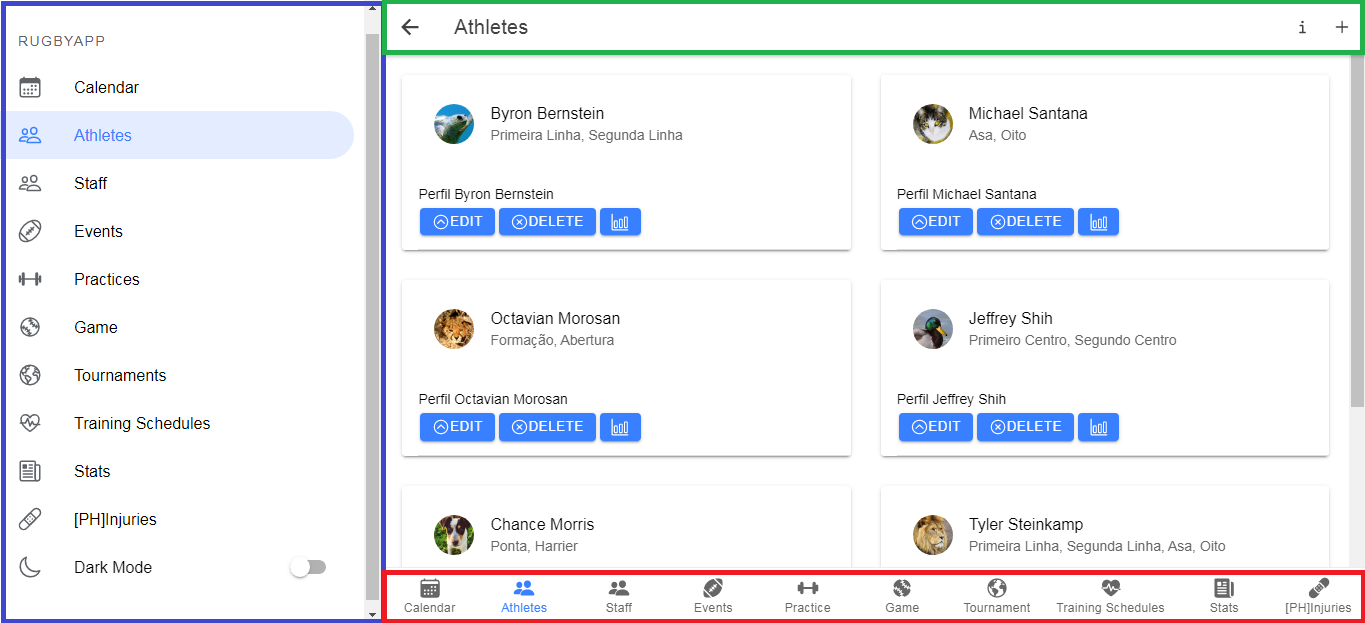
\includegraphics{./figures/frontend/MainComponent.png}}
	\end{center}
	\caption{Vista inicial da aplicação. Observa-se o \textit{ion-split-pane} a azul, o \textit{ion-tabs} a vermelho e o \textit{ion-header} a verde.}\label{fig:maincomponent}
\end{figure}

Como mencionado na secção 4.1.1, existem páginas na nossa aplicação cliente que requerem mais do que um \textit{Component} para garantir certas regras de negócios sem que a informação nas páginas fique sobrelotada e proporcionando a melhor experiência de utilização. Existem componentes na \textit{API} do \textit{Ionic} (alguns também mencionados na secção 4.1.1) que foram utilizados para este mesmo propósito:\\

\begin{tabular}{ll}
	\textit{ion-modal} & \textit{Dialog} (componente visual que se sobrepõe ao contexto atual da página e \\
	&requer interação do utilizador para desaparecer), normalmente utilizado \\
	&para apresentar uma página onde o utilizador tem diversas opções de interação.
	\\
	\textit{ion-popover} & \textit{Dialog} (assim como o \textit{ion-modal}) que é geralmente usado para conter acções \\
	&ou informação que não pode ser mostrada na totalidade sem comprometer\\
	& visualmente os elementos da página.
	\\
	\textit{ion-select} & Apesar de não requerer um \textit{controller} ou um \textit{component} próprio para ser \\
	&programado, o \textit{ion-select} é um \textit{ion-modal} pré-definido na \textit{API} exclusivamente \\
	&para \textit{input}/\textit{output} (ou seja, não é possível atribuir-lhe diretamente outro \\
	&comportamento que não o de dar ao utilizador diversas opções de escolha).
\end{tabular}

\begin{figure}[h]
	\begin{center}
		\resizebox{150mm}{!}{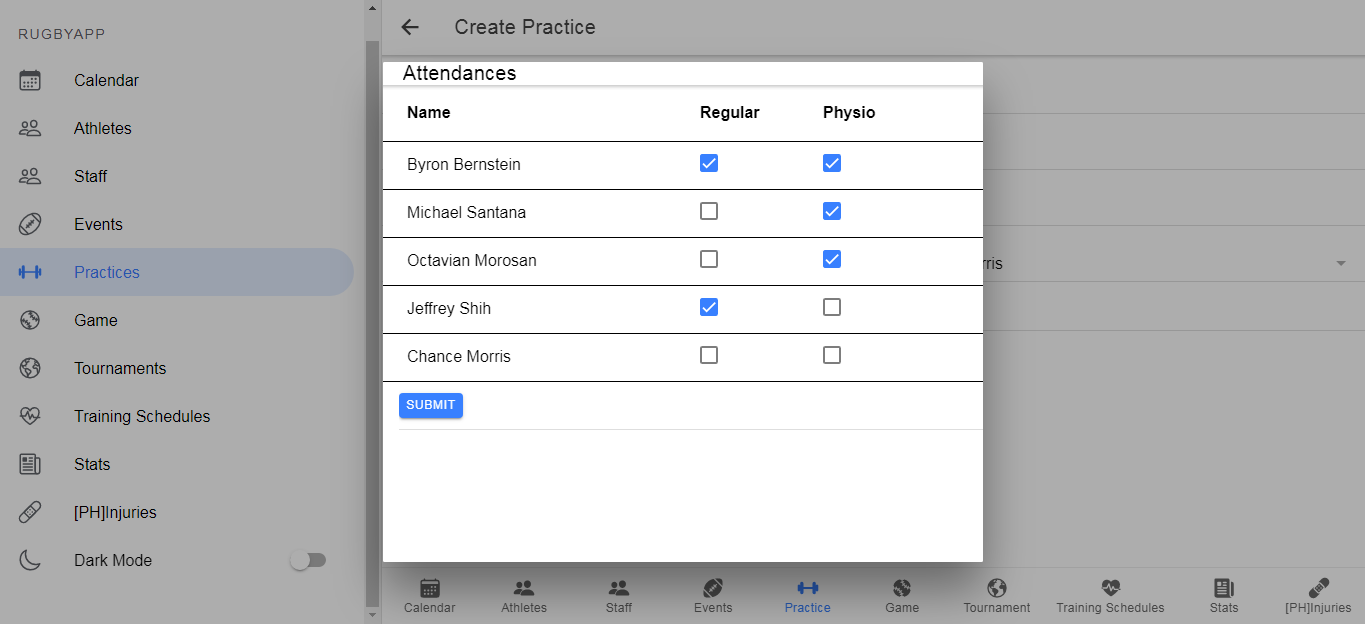
\includegraphics{./figures/frontend/PracticeFormPopover.png}}
	\end{center}
	\caption{\textit{Modal} da página do formulário de \textit{Practice}.}\label{fig:practiceformmodal}
\end{figure}
\newpage

\begin{figure}[h]
	\begin{center}
		\resizebox{150mm}{!}{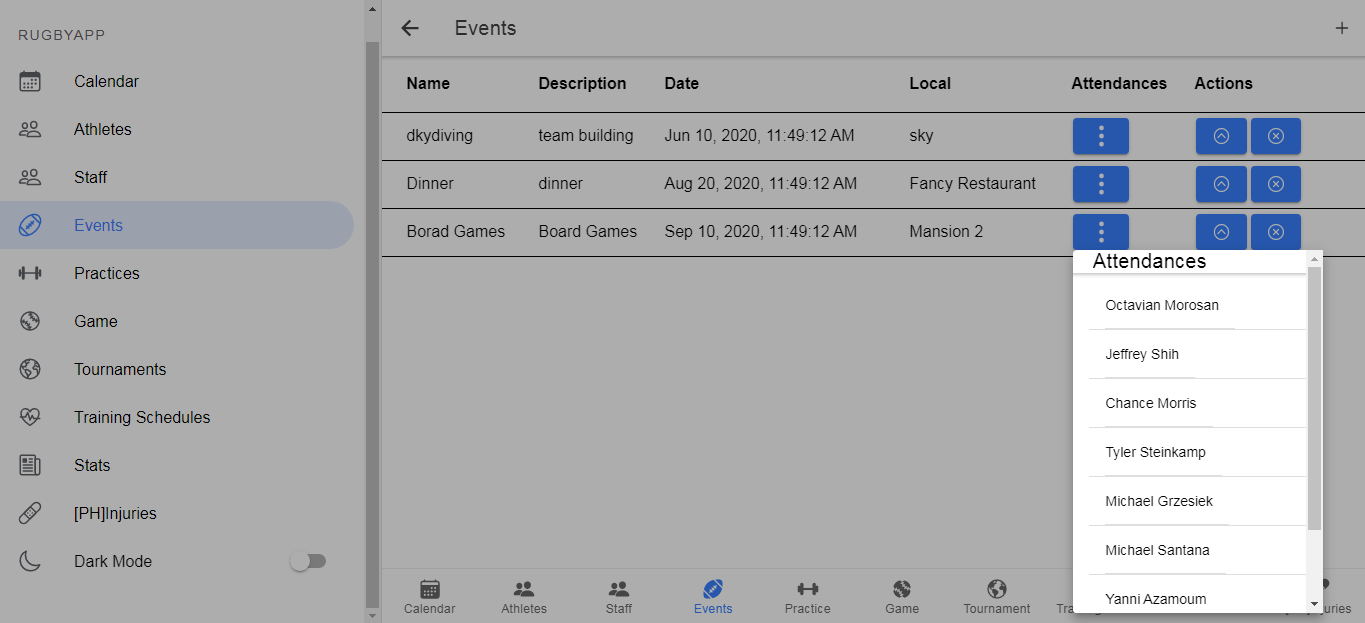
\includegraphics{./figures/frontend/EventPopover.png}}
	\end{center}
	\caption{\textit{Popover} da página \textit{Event}.}\label{fig:eventpopover}
\end{figure}

\begin{figure}[h]
	\begin{center}
		\resizebox{150mm}{!}{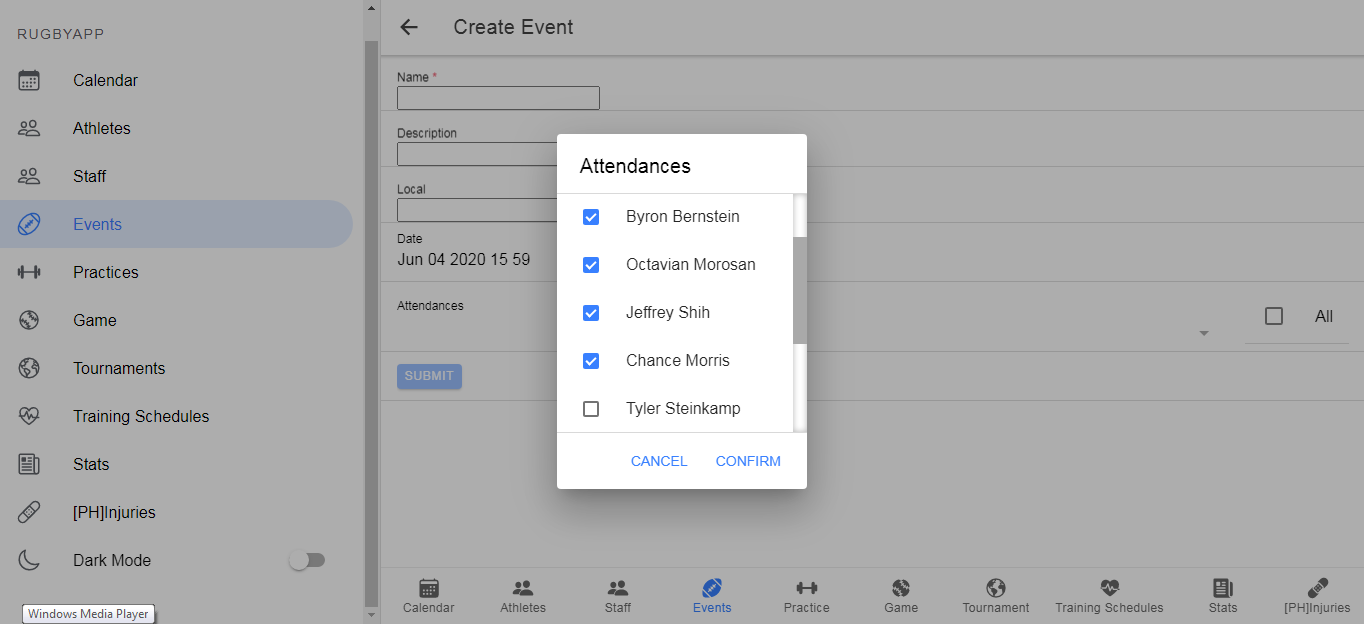
\includegraphics{./figures/frontend/EventFormSelect.png}}
	\end{center}
	\caption{\textit{Select} da página do formulário de \textit{Event}.}\label{fig:eventformselect}
\end{figure}
 \newpage
 
Como referido anteriormente, ao contrário do \textit{ion-select}, o \textit{ion-modal} e o \textit{ion-popover} são componentes próprios e requerem um \textit{controller} para serem gerados e criados por outros componentes. Podemos observar no troço de código seguinte, o método \textit{createPopover()} inserido no \textit{event.component}

\begin{lstlisting}
constructor(private eventService: EventService, private popoverController: PopoverController, private alertController: AlertController) { }

/* . . .*/

async createPopover(profiles: Profile[], ev) {
	const popover = await this.popoverController.create({
		component: EventPopoverComponent,
		componentProps: { profiles },
		event: ev
	});
	return await popover.present();
}
\end{lstlisting}



O \textit{Component event.component} importa o módulo \textit{PopoverController} do \textit{package} do \textit{Ionic}, e cria a sua instância no construtor. Atribuindo o método \textit{createPopover} a um evento, é assim invocada a criação de um \textit{Popover}. 

\begin{lstlisting}
<ng-container matColumnDef="profiles">
	<th mat-header-cell *matHeaderCellDef> Attendances </th>
	<td mat-cell *matCellDef="let element">
		<ion-button (click)="createPopover(element.profiles,$event)">
			<ion-icon slot="icon-only" name="ellipsis-vertical"></ion-icon>
		</ion-button>
	</td>
</ng-container>
\end{lstlisting}



Cada elemento da coluna de \textit{Attendances} tem o seu próprio botão que vai criar o seu próprio \textit{Popover}. Passando a lista de \textit{Profiles} associadas a cada elemento, podemos criar um \textit{Popover} com cada uma das listas de \textit{Profiles} na tabela da página \textit{Event}.\\

\begin{lstlisting}
<ion-content>
	<ion-list>
		<ion-item *ngFor="let profile of this.navParams.get('profiles')">
			/* . . . */
		</ion-item>
	</ion-list>
</ion-content>
\end{lstlisting}

Através de um módulo existente no package do \textit{Ionic}, chamado \textit{NavParams}, é possível passar informação ao \textit{Controller} do \textit{Popover}, e é possível do lado do \textit{Popover} obter essa informação para ser consumida. Neste caso, o Popover é meramente uma lista de itens com os nomes dos \textit{Profiles}, com um \textit{Link} para a página desse \textit{Profile}.

Do lado do \textit{ion-modal}, a ideia-chave é idêntica, exceto que o módulo que é importado pelo \textit{component} passa a ser o \textit{ModalController} em vez de \textit{PopoverController}. Continua-se a usar o \textit{NavParams} para passar informação ao \textit{Modal}.

\subsection{Angular Materials CDK}

O \textit{Angular} tambem dispõe de um \textit{CDK} (\textit{Component Dev Kit}) chamado \textit{Angular Materials}, onde encontramos vários componentes visuais. Em [2] podemos encontrar a lista completa de todos os componentes disponíveis neste \textit{CDK}. Apesar da nossa aplicação cliente explorar maioritariamente componentes da \textit{IONIC API}, também são usados alguns componentes deste \textit{CDK}, nomeadamente\\

\begin{tabular}{ll}
	\textit{mat-table} & Tabela usada para mostrar dados em diversas páginas da nossa \\
	&aplicação cliente, com a possibilidade de 
	adicionar comportamentos \\
	&adicionais à tabela, como paginação, linha de rodapé, filtro e ordenação. \\
	& \\
	\textit{mat-grid-list} & Grelha que permite variar os tamanhos que cada item ocupa na grelha,\\
	& ambos em número de colunas ou número de linhas, criando dinamismo \\
	&na organização da grelha sem a comprometer visualmente.\\
	& \\
	\textit{mat-form-field} & Componente que representa o campo de um formulário, onde se podem \\
	&aplicaram estilos de texto como \textit{Placeholder}, \textit{Hint} ou texto de erro. \\
	&(Exemplificado na sub-secção 4.28)\\
\end{tabular}

Podemos observar no excerto de código seguinte o \textit{template} da \textit{mat-table} de \textit{Games}.

\begin{lstlisting}
<ion-content>
	<table mat-table [dataSource]="this.dataSource" matSort class="mat-elevation-z8">
	
		<ng-container matColumnDef="date">
			<th mat-header-cell *matHeaderCellDef mat-sort-header> Date </th>
			<td mat-cell *matCellDef="let element"> {{element.date | date:"medium"}} </td>
		</ng-container>
		
		/* . . . */
		
		<tr mat-header-row *matHeaderRowDef="displayedColumns"></tr>
		<tr mat-row *matRowDef="let row; columns: displayedColumns;"></tr>
	</table>
</ion-content>
\end{lstlisting}
As \textit{mat-table} do \textit{Angular Materials} funcionam com base num objeto \textit{DataSource}. O \textit{Component} principal de cada página tem uma propriedade com este objeto, e após fazer \textit{data-fetching}, afeta esta propriedade com a informação para popular a tabela com os dados. Cada \textit{Component} tem também um \textit{array} com o nome das colunas da tabela. Da forma que o \textit{mat-table} é implementado, podemos organizar os nomes neste \textit{array} com a ordem que se pretende que as colunas sejam apresentados visualmente, e a tabela será desenhada com essa ordem, independentemente da ordem como está definido o HTML de cada coluna. \\


\begin{lstlisting}
export class GameComponent implements OnInit {
	games: Game[];
	displayedColumns: string[] = ['date', 'local', 'opponent', 'score', 'comment', 'athletes', 'actions'];
	dataSource: any;
	@ViewChild (MatSort, {static: true}) sort: MatSort;

	/* . . . */

	showGames() {
		this.gameService.getGames().subscribe(games => {
			this.games = games;
			this.dataSource = new MatTableDataSource(this.games);
			this.dataSource.sort = this.sort;
		});
	}
	/* . . . */
}
\end{lstlisting}

\begin{figure}[h]
	\begin{center}
		\resizebox{150mm}{!}{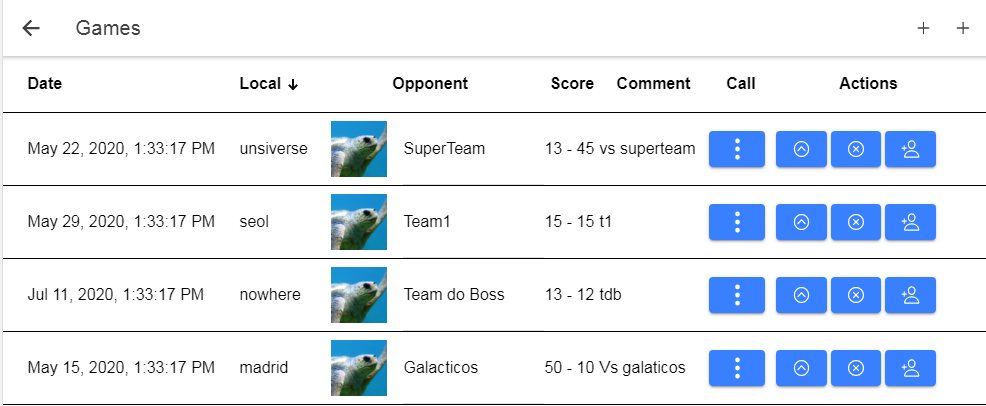
\includegraphics{./figures/frontend/GamesSortedNameDown.png}}
	\end{center}
	\caption{Tabela da página de \textit{Games}, ordenada decrescentemente por nome.}\label{fig:gamessortednameup}
\end{figure}



No que toca ao \textit{mat-grid-list}, podemos observar no troço de código seguinte como é que este componente é utilizado no \textit{Profile} de um \textit{Staff}.
\\

\begin{lstlisting}
<mat-grid-list cols="3" rowHeight="100px">
	<mat-grid-tile [colspan]="1" [rowspan]="3">
		<img [src]="staff?.profile.photo">
	</mat-grid-tile>
	
	<mat-grid-tile [colspan]="2" [rowspan]="1">
		<ion-label>
			<div class="ion-text-center"> <b> Nome </b> </div>
			<div class="ion-text-center"> {{staff?.profile.name}} </div>
		</ion-label>
	</mat-grid-tile>
	
	/* . . . */
</mat-grid-list>

\end{lstlisting}

Como referido anteriormente, uma das características chave do \textit{mat-grid-list} é a possibilidade de atribuir tamanhos diferentes aos diferentes items da grelha, permitindo-os organizar visualmente enquanto se mantem as proporções corretas da tabela. 

\begin{figure}[h]
	\begin{center}
		\resizebox{150mm}{!}{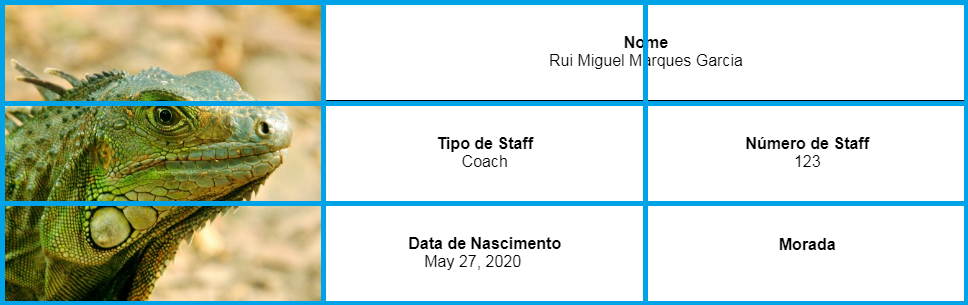
\includegraphics{./figures/frontend/StaffProfile.png}}
	\end{center}
	\caption{\textit{Profile} de um \textit{Staff}, com as linhas da grelha \textit{highlighted} para fins de visualização. }\label{fig:calendarall}
\end{figure}

É possível aferir, com base na imagem anterior, que a grelha gerada é uma grelha 3x3, no entanto, o item da imagem do perfíl ocupa 1x3, o nome do perfíl ocupa 2x1, e os restantes itens ocupam 1x1. É possível também aferir, apesar dos tamanhos variados, que a grelha fica organizada e ocupa espaço proporcional em ambos os eixos.

\subsection{Classes e Entidades}

Foram geradas na aplicação cliente as classes correspondentes às entidades da aplicação servidora em \emph{TypeScript}. Podemos observar no troço de código seguinte, como exemplo, a classe \emph{Event.ts} inserida no \emph{package} de classes da nossa Aplicação Cliente.

\begin{lstlisting}
import {Profile} from './profile';

export class Event {
	constructor(
		private id?: number,
		private name?: string,
		private description?: string,
		private date?: Date,
		private local?: string,
		private profiles?: Profile[]
	) {
		this.id = id ? id : 0;
		this.description = description ? description : '';
		this.date = date ? date : new Date(0);
		this.local = local ? local : '';
		this.name = name ? name : '';
		this.profiles = profiles ? profiles : [];
	}
}
\end{lstlisting}

Um dos aspetos principais a salientar na implementação dos construtores das Entidades na aplicação cliente é a questão das propriedades poderem ser \emph{nullable}. Organizando os construtores para que todas as propriedades sejam \emph{nullable} enquanto se faz a verificação no corpo do construtor para a ausência destas propriedades, permite-se construir objetos atribuindo valores padrão a todas as propriedades que não existem na altura da criação. Este detalhe de implementação ajuda a gerar objetos vazios sem os problemas que ocorrem frequentemente na manipulação de valores \emph{null}.

\section{Descrição das Páginas}\label{sec42}

Esta secção aborda os componentes das diversos páginas implementados na aplicação cliente. No apêndice B é observável um diagrama em árvore da navegação da aplicação cliente.

\subsection{\textit{Calendar}}\label{subsec422}

O \textit{Calendar}, referido nesta sub-secção como Calendário, é a página principal da aplicação cliente. É a primeira página a ser mostrada quando um utilizador entra na aplicação. 

\begin{figure}[h]
	\begin{center}
		\resizebox{120mm}{!}{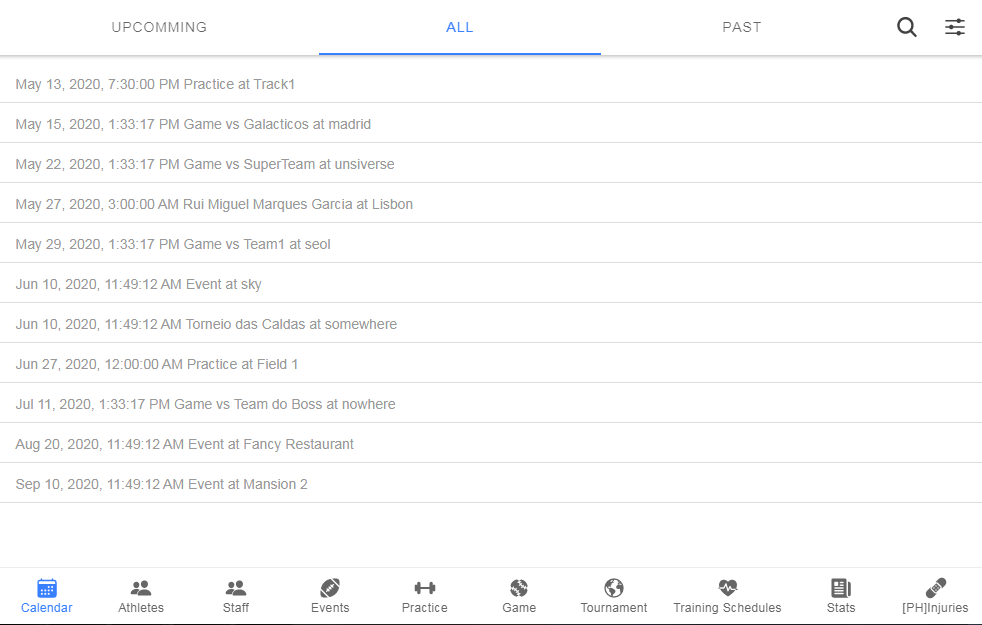
\includegraphics{./figures/frontend/CalendarAll.png}}
	\end{center}
	\caption{Aba \textit{All} do Calendário.}\label{fig:calendarall}
\end{figure}

O Calendário mostra todas as entradas de \textit{Games}, \textit{Events}, \textit{Practices} e \textit{Tournaments}, através da sua data e localização.

O Calendário contem as abas \textit{Upcomming}, \textit{All} e \textit{Past}. A aba \textit{Upcomming} mostra todas as entradas que irão decorrer nos próximos N dias, sendo o valor por omissão de N 15 dias. No menu de filtro existe um campo onde é possível aumentar ou diminuir este valor de N, consoante a informação que se quer mostrar. A aba \textit{Past} mostra todas as entradas cuja data de concretização já ocorreu. A aba \textit{All} mostra todas as entradas. No caso da aba Upcomming, o calendário também mostra o tempo, em semanas, dias, horas, e minutos, até a entrada de concretização.

\begin{figure}[h]
	\begin{center}
		\resizebox{120mm}{!}{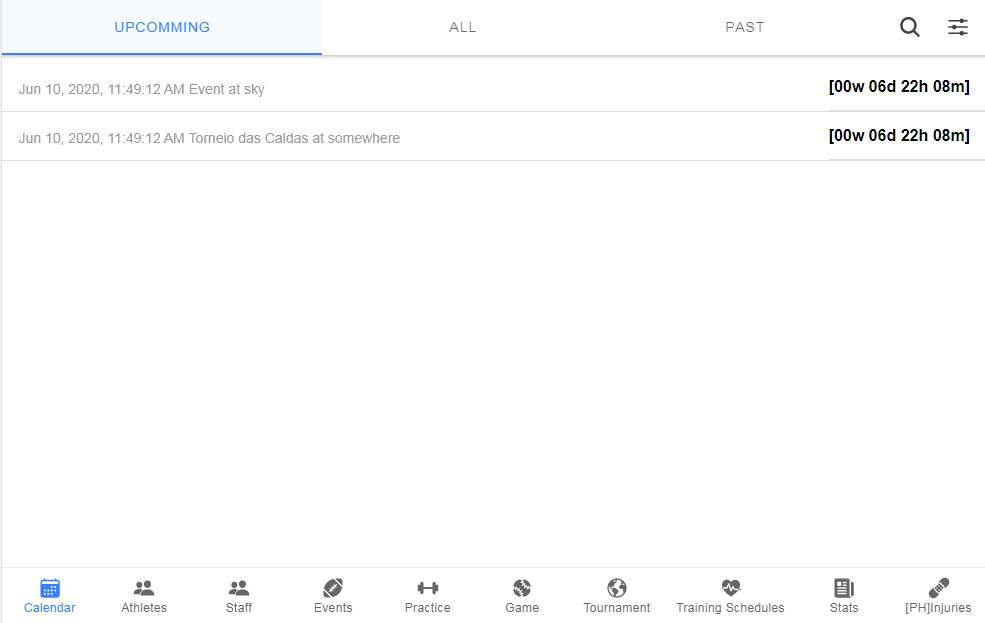
\includegraphics{./figures/frontend/CalendarUpcomming.png}}
	\end{center}
	\caption{Aba \textit{Upcomming} do Calendário.}\label{fig:calendarupcomming}
\end{figure}

O Calendário implementa uma barra de pesquisa, que pesquisa por nome, local ou oponente (caso se aplique), e apresenta apenas as entradas encontradas nessa pesquisa. Esta pesquisa é aplicada às três abas do Calendário.

\begin{figure}[h]
	\begin{center}
		\resizebox{120mm}{!}{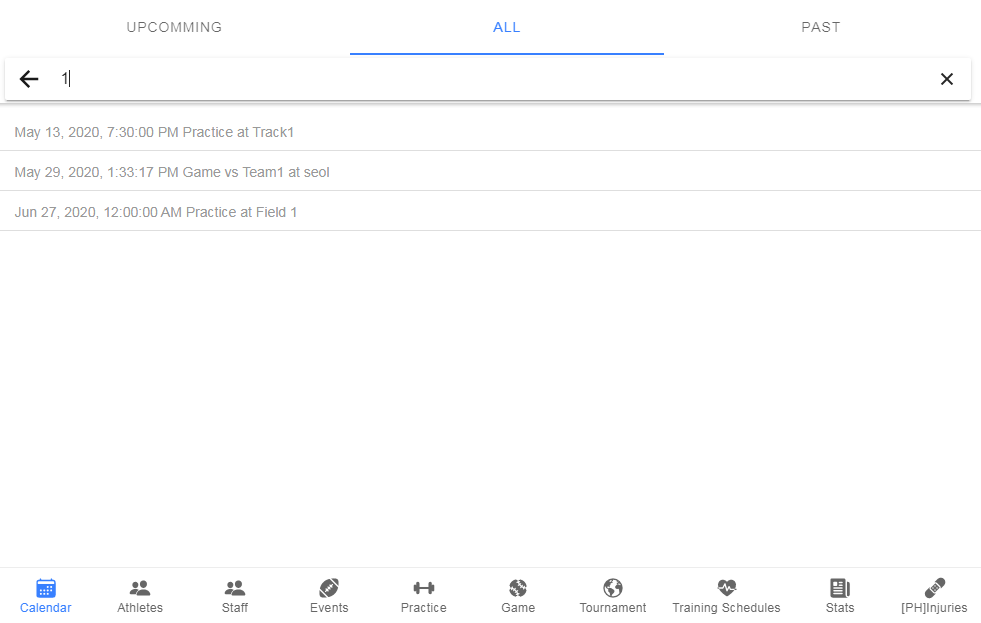
\includegraphics{./figures/frontend/CalendarSearchBar.png}}
	\end{center}
	\caption{Barra de pesquisa do Calendário. A pesquisa pela \textit{string} "1" mostra todas as entradas onde o nome, local ou oponente contém essa \textit{string}. }\label{fig:gamessortednameup}
\end{figure}

O Calendário implementa um menu de filtros, que permite filtrar por \textit{Games}, \textit{Events}, \textit{Practices} ou \textit{Tournaments}. Este filtro é aplicado às três abas do Calendário. Como referido anteriormente, tambem permite filtrar o número de dias de alcance da aba \textit{Upcomming}.
\newpage


\subsection{\textit{Athletes/Staff}}\label{subsec423}

Ao contrário dos restantes componentes, a página de \textit{Athletes} e \textit{Staff} é apresentada utilizando uma listagem diferente. Foi decidido que, dado que uma lista de atletas e \textit{staff} apresenta informação que é , visualmente, mais facilmente perceptivél utilizando as fotografias dos perfís, optá-mos por fazer uma grelha com \textit{ion-cards}. Um \textit{ion-card} serve essencialmente como uma peça visual que agrupa a informação mais importante sobre um perfíl, e serve de ponto de entrada para informação mais detalhada. Podemos utilizar uma colecção de \textit{ion-cards} para agrupar toda a informação que é mais relevante numa lista de atletas sem obrigar o utilizador a entrar para dentro de um perfíl.
\newpage

\begin{figure}[h]
	\begin{center}
		\resizebox{150mm}{!}{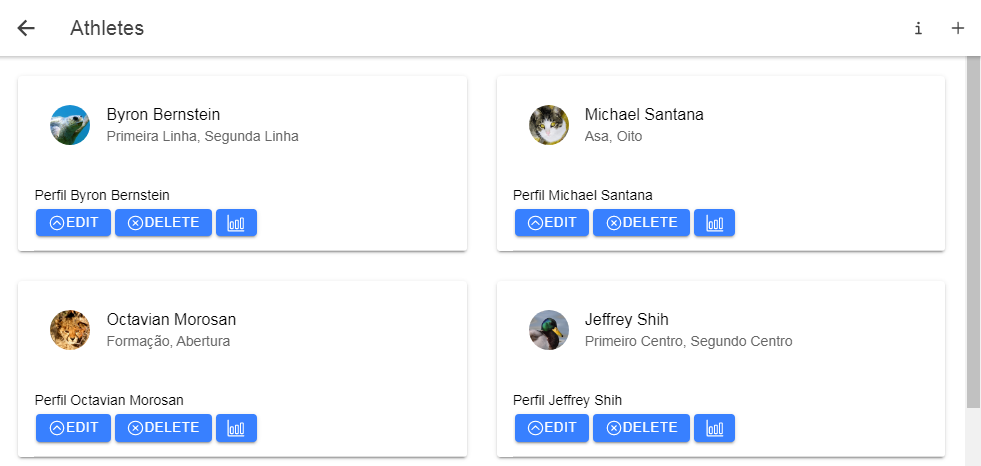
\includegraphics{./figures/frontend/AthleteList.png}}
	\end{center}
	\caption{Página da lista de \textit{Athletes}.}\label{fig:athletelist}
\end{figure}


\subsection{\textit{Profile}}\label{subsec424}
A página de \textit{Profile} é também diferenciada das outras páginas da aplicação cliente, por não mostrar uma lista de entidades, mas sim todos os dados de uma entidade específica. 
Foi decidido, como referido na sub-secção 4.1.6, usar-se uma \textit{mat-grid-list} para implementar os perfís de atletas e equipa técnica, pois a \textit{mat-grid-list} é um grelha que facilita a organização de colunas e linhas, sendo possível expandir umas e encolher outras sem comprometer visualmente a grelha. 
\begin{figure}[h]
	\begin{center}
		\resizebox{100mm}{!}{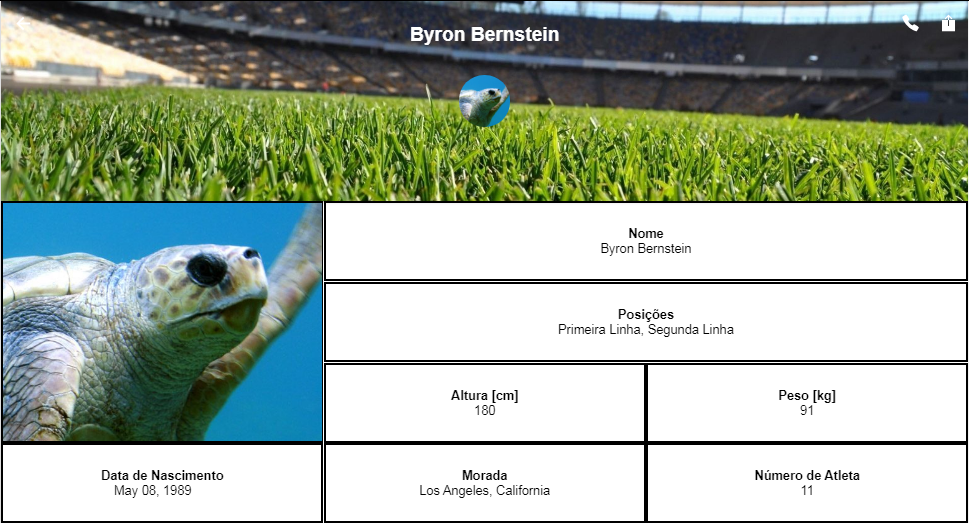
\includegraphics{./figures/frontend/AthleteProfile.png}}
	\end{center}
	\caption{Página do \textit{Profile} de um \textit{Athlete}.}\label{fig:athleteprofile}
\end{figure}

O perfil de um atleta organiza assim, numa grelha 3x4, toda a informação do atleta. Também se observa, no cabeçalho do perfil, uma imagem de fundo (\textbf{irá ser alterada no futuro}), e os botões de \textit{Contact}, com o e-mail e o número de telefone do atleta para fins de entrar em contacto com este, assim como um \textit{Share} (\textbf{não implementado}).



\subsection{\textit{AthleteStats}}\label{subsec425}
A página de estatísticas de atleta é também diferenciada das restantes páginas com tabelas por conter uma tabela com maior dimensão, dada a carga de dados que tem de apresentar. Nesta página em particular, o \textit{split-pane} é escondido manualmente pela aplicação, para conseguir manter a tabela toda no ecrã. 

\begin{lstlisting}
ionViewDidEnter() {
	this.menuController.enable(false, 'main-menu');
}

ionViewDidLeave() {
	this.menuController.enable(true, 'main-menu');
}
\end{lstlisting}
Para entender melhor estes métodos, é explicado em seguida o \textit{Ionic Lifecycle} de cada componente. Este \textit{lifecycle} segue a seguinte estrutura ordenada\\

\begin{tabular}{ll}
	\textit{constructor} & É executado quando a página é iniciada. É o melhor sitio \\
	&para definir valores \textit{default} para as nossas variáveis.\\
	\textit{ionViewDidLoad} & É executado quando a página foi carregada. Este evento é só \\
	&executado uma vez por cada criação de cada página. Se a página \\
	&for recarregada mas estiver em \textit{cache}, este evento não é executado\\
	& outra vez.\\
	\textit{ionViewWillEnter} & É executado quando a página está prestes a entrar e a tornar-se \\
	&a página ativa.\\
	\textit{ionViewDidEnter} & É executado quando a página entrou por completo e é agora a \\
	&página ativa. Este evento é sempre executado, independemente de \\
	&ser o primeiro carregamento da página ou se a página for \\
	&carregada da \textit{cache}.\\
	\textit{ionViewWillLeave} & É executado quando a página está prestes a sair e deixar de ser \\
	&a página ativa.\\
	\textit{ionViewDidLeave} & É executado quando a página acabou de sair e já não é a \\
	&página ativa.\\
	\textit{ionViewWillUnload} & É executado quando a página está prestes a ser destruída e os \\
	&seus elementos a serem removidos.\\
	\\
\end{tabular}

É possível, através deste \textit{Lifecycle}, definir quando é que alguns comportamentos são executados. Neste caso, o \textit{split-pane} é escondido no gancho \textit{ionViewDidEnter}
e volta a ser mostrado no gancho \textit{ionViewDidLeave}.

Como esta tabela contem um elevado número de colunas, foram usadas siglas para o nome de cada coluna. No canto superior direito do cabeçalho da página, encontramos o botão \textit{Subtitles}, que abre um menu lateral com a legenda da tabela. 
\newpage

\begin{figure}[h]
	\begin{center}
		\resizebox{120mm}{!}{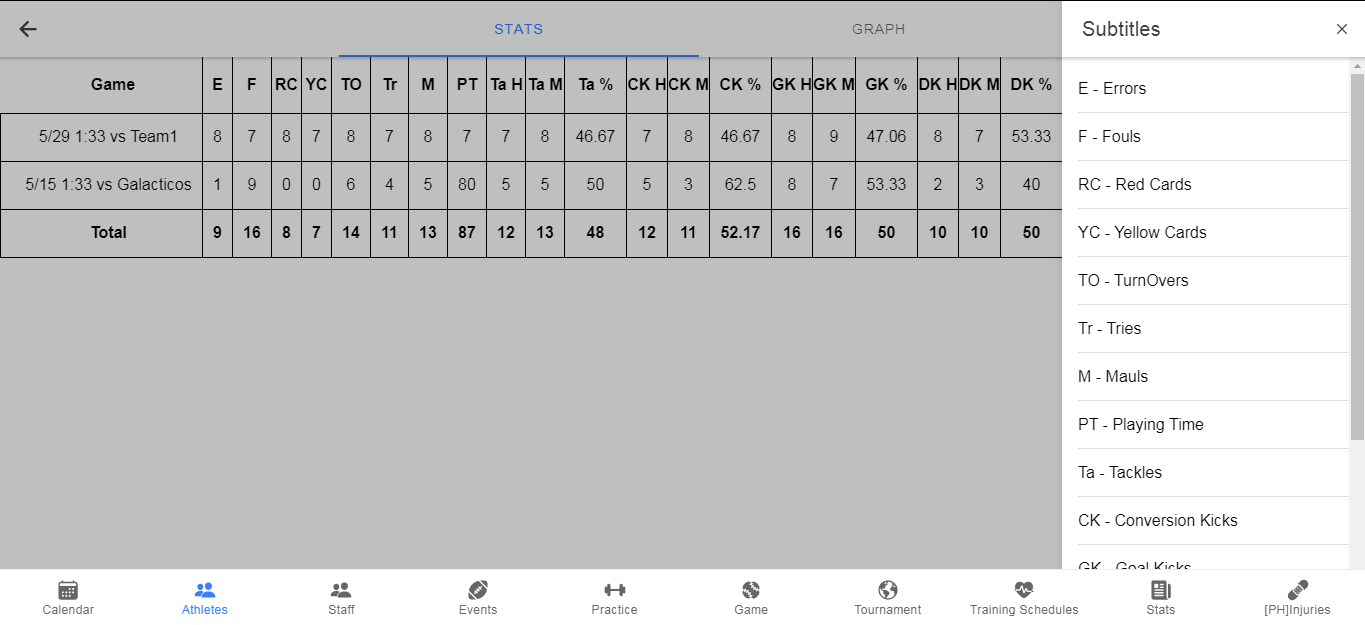
\includegraphics{./figures/frontend/AthleteStatsSubtitles.png}}
	\end{center}
	\caption{Página da tabela \textit{AthleteStats} com o menu da legenda aberto.}\label{fig:athleteprofile}
\end{figure}

Existe também nesta página uma aba de \textit{Graphs}, que mostra através de gráficos a mesma informação que a aba \textit{Stats}.

A geração de gráficos é feita com base numa biblioteca chamada \textit{Chart.js}. \textit{Chart.js} é uma bibliteca \textit{open-source} com o foco príncipal em criar grafos responsivos. Em [3] encontramos a referência para esta biblioteca. 

Esta biblioteca contem a implementação de um objeto \textit{Chart}, que recebe, entre outra informação, o tipo de gráfico, as \textit{labels}, algumas opções de renderização, e \textit{Data Sets}. Cada \textit{Data Set} representa um bloco de informação no gráfico (no caso de um gráfico de barras, cada barra é um \textit{data set}, no caso de um gráfico de linhas, cada linha é um \textit{data set}).

No que toca a questões de experiência de utilização, a nossa interface de gráficos é baseada em \textit{checkboxes}. Cada gráfico contem um \textit{menu} de \textit{checkboxes}, onde o utilizador pode escolher que estatísticas quer adicionar ou remover do gráfico, adicionando ou removendo o \textit{dataset} dessa estatística ao \textit{array} do \textit{graph}. 

\begin{figure}[h]
	\begin{center}
		\resizebox{130mm}{!}{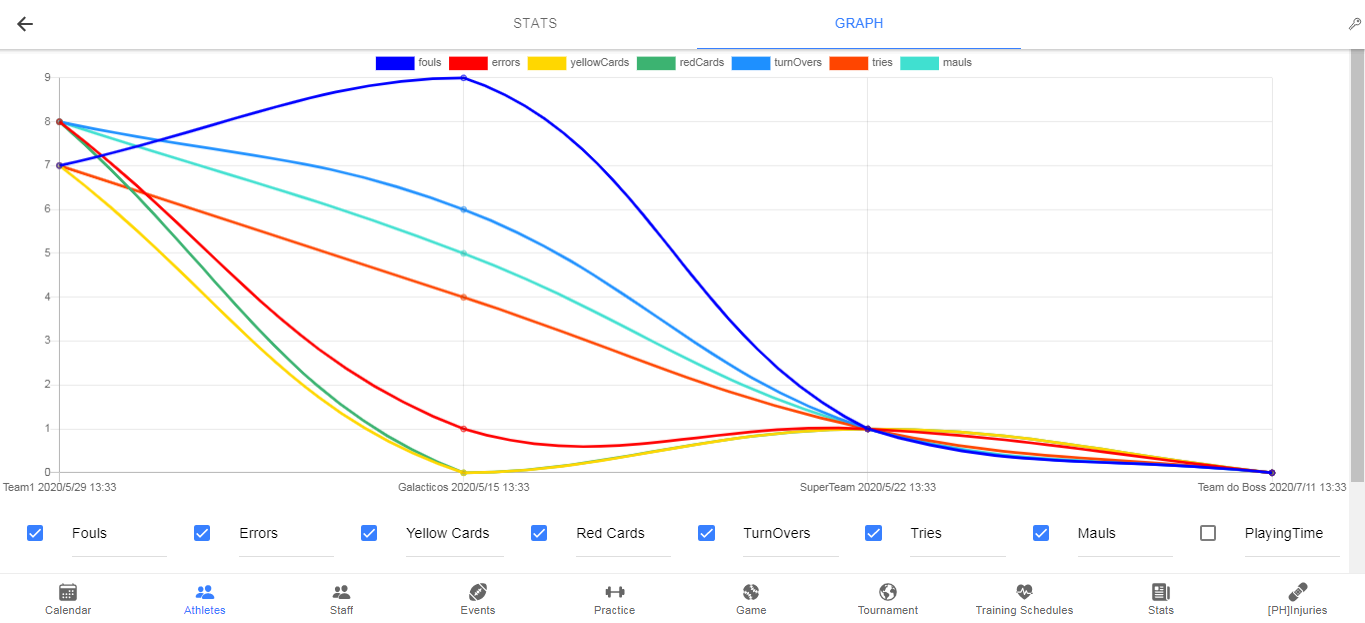
\includegraphics{./figures/frontend/graph.png}}
	\end{center}
	\caption{Aba \textit{Graph}, com as estatísticas \textit{Fouls}, \textit{Errors}, \textit{YellowCards}, \textit{RedCards}, \textit{turnOvers}, \textit{tries} e \textit{mauls} selecionados.}\label{fig:athleteprofile}
\end{figure}
\newpage

\subsection{\textit{Events/Practices/Games/Tournaments/TrainingSchedules}}\label{subsec426}
Estas cinco páginas são todas idênticas na sua estrutura, pois são as páginas que apresentam as tabelas das diferentes entidades.
Como foi mencionado na sub-secção 4.1.5, estas páginas implementam todas uma \textit{mat-table} ordenável com a informação das entidades. Dependendo do contexto das entidades, existem botões em cada linha com um \textit{Popover} com a lista de participantes/presenças/convocados, e uma coluna de Acções, onde estão os botões de \textit{Edit} e \textit{Delete}.

\begin{figure}[h]
	\begin{center}
		\resizebox{120mm}{!}{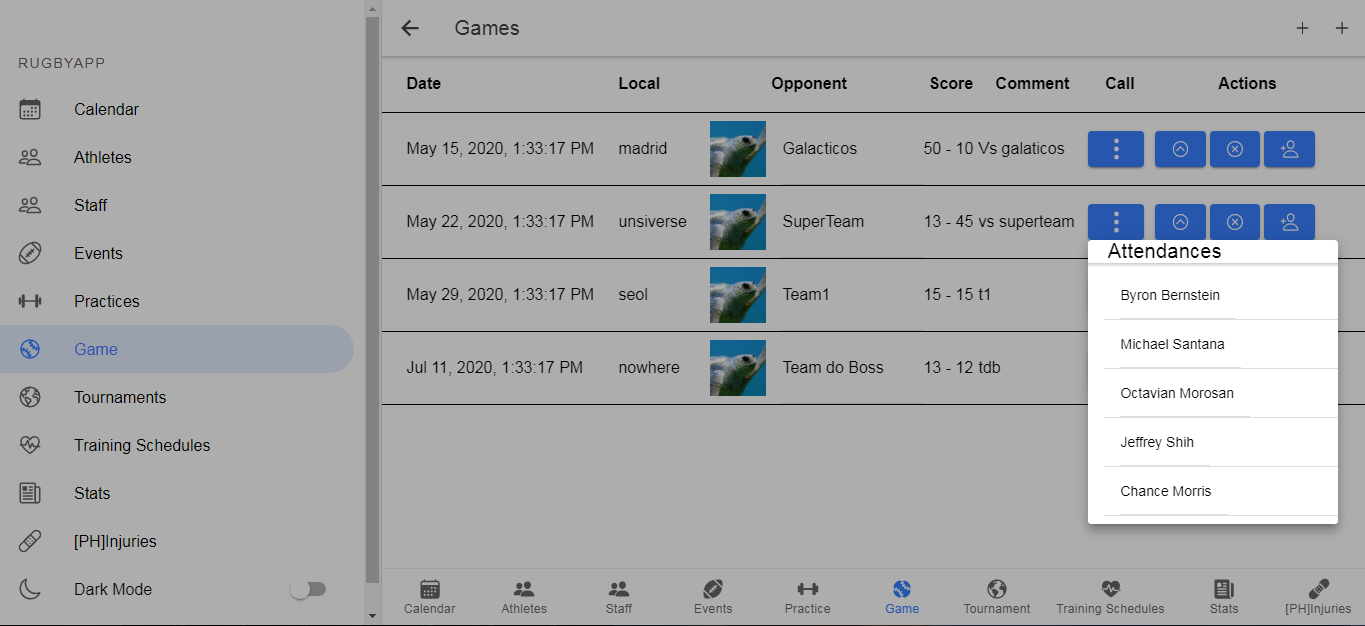
\includegraphics{./figures/frontend/GamePopover.png}}
	\end{center}
	\caption{Figura da página da tabela \textit{Games}, com o \textit{Popover} aberto a mostrar os Convocados.}\label{fig:athleteprofile}
\end{figure}
A página de \textit{Games} apresenta uma diferença distinta para todos os outros: o \textit{ActiveRoster}. O \textit{ActiveRoster} serve para definir os titulares no contexto de um jogo. O botão de \textit{Add Active Roster} leva o utilizador para um formulário específico, onde são apresentadas as posições que os jogadores de Rugby podem cumprir, e cada posição abre um \textit{ion-select} com uma lista filtrada de atletas que jogam naquela posição.

\begin{figure}[h]
	\begin{center}
		\resizebox{120mm}{!}{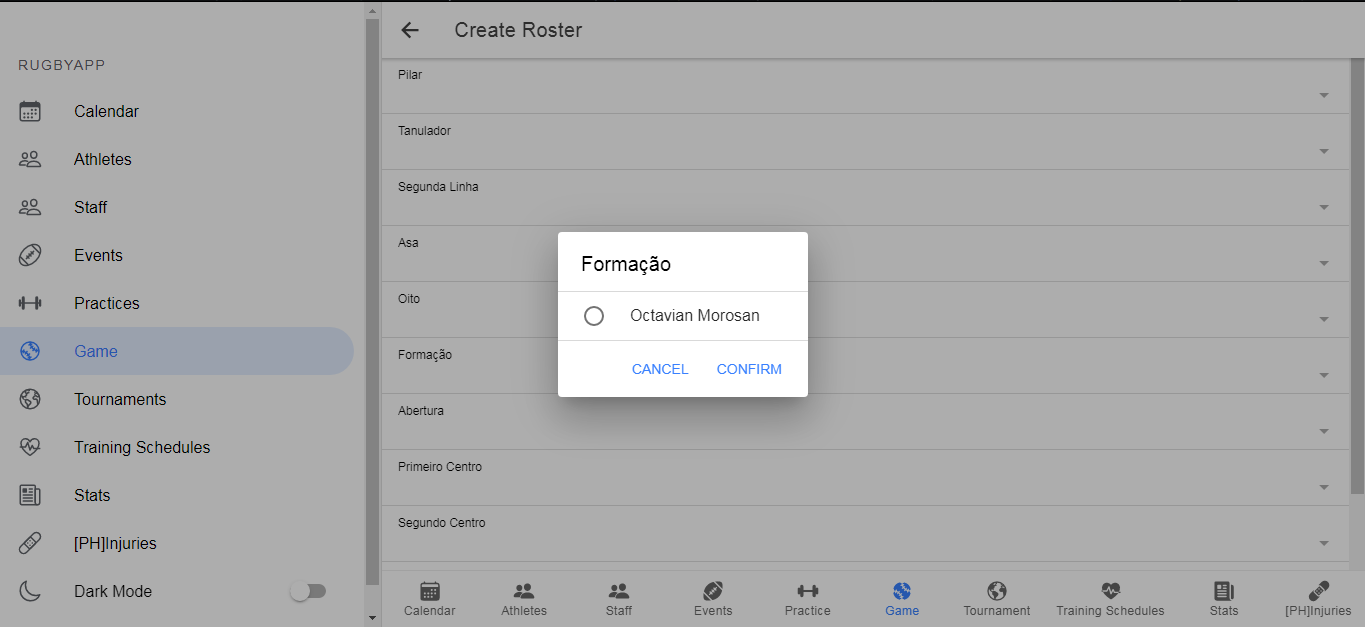
\includegraphics{./figures/frontend/ActiveRoster.png}}
	\end{center}
	\caption{Página da tabela \textit{ActiveRoster}, com a posição "Formação" selecionada, e o \textit{ion-select} a mostrar a lista filtrada de atletas que jogam naquela posição.}\label{fig:athleteprofile}
\end{figure}
\newpage

\begin{figure}[h]
	\begin{center}
		\resizebox{150mm}{!}{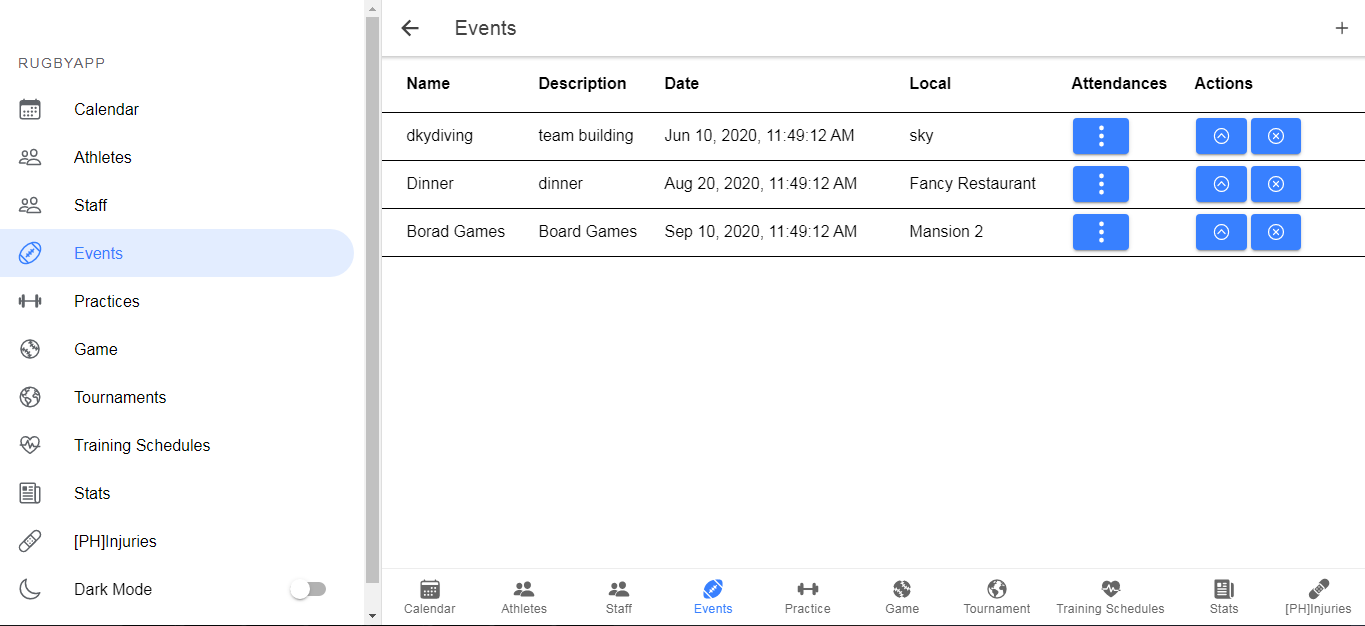
\includegraphics{./figures/frontend/Events.png}}
	\end{center}
	\caption{Página da tabela \textit{Events}.}\label{fig:events}
\end{figure}

\begin{figure}[h]
	\begin{center}
		\resizebox{150mm}{!}{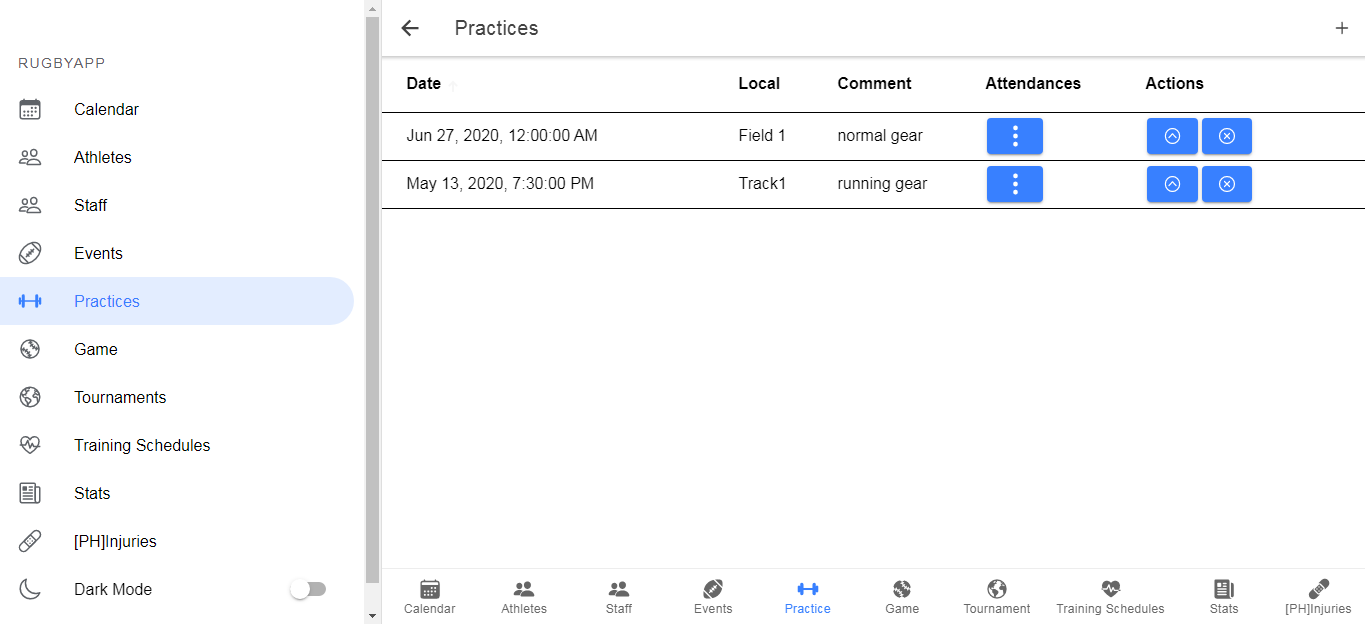
\includegraphics{./figures/frontend/Practices.png}}
	\end{center}
	\caption{Página da tabela \textit{Practices}.}\label{fig:practices}
\end{figure}
\newpage

\begin{figure}[h]
	\begin{center}
		\resizebox{150mm}{!}{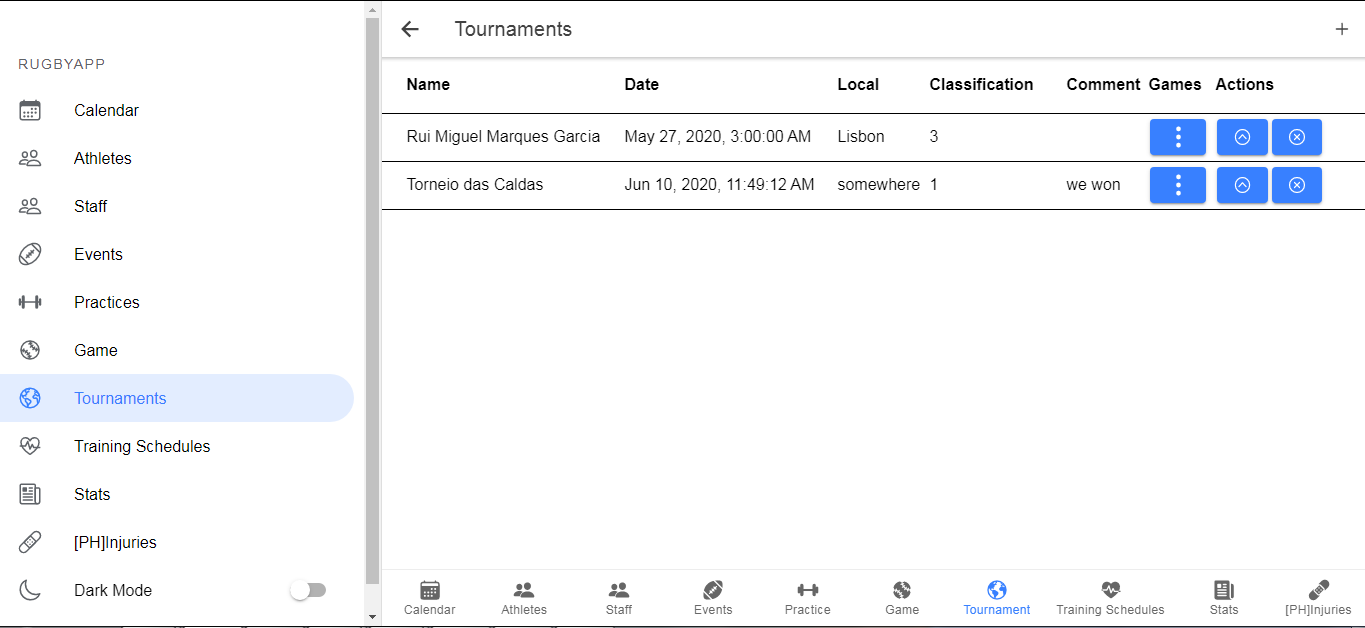
\includegraphics{./figures/frontend/Tournaments.png}}
	\end{center}
	\caption{Página da tabela \textit{Tournaments}.}\label{fig:tournaments}
\end{figure}
\begin{figure}[h]
	\begin{center}
		\resizebox{150mm}{!}{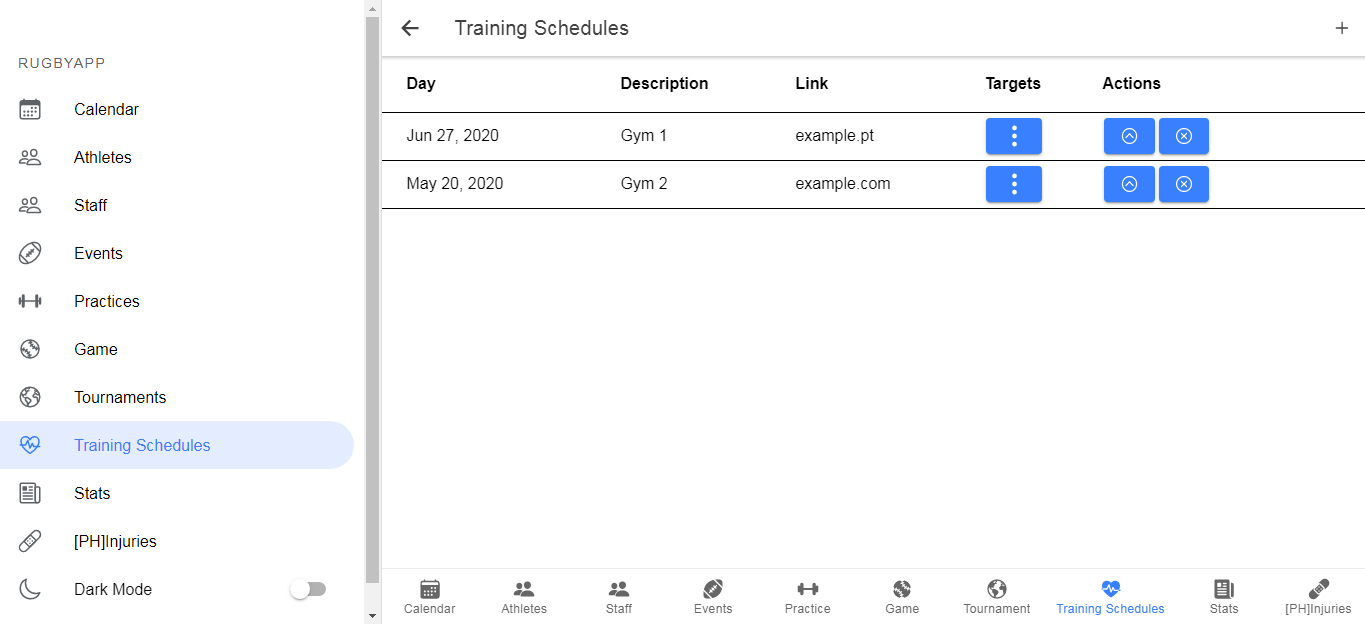
\includegraphics{./figures/frontend/TrainingSchedules.png}}
	\end{center}
	\caption{Página da tabela do \textit{TrainingSchedules}.}\label{fig:athleteprofile}
\end{figure}
\newpage

\subsection{\textit{GameStats}}\label{subsec427}
A página de \textit{GameStats} é a página principal das estatísticas de jogo. Enquanto que o \textit{AthleteStats} mostra as estatísticas associadas a um jogador, o \textit{GameStats} mostra e deixa adicionar estatísticas associadas a um jogador num jogo.

Esta página apresenta a lista de jogos, similarmente à lista de \textit{Athletes} ou \textit{Staff}, através duma grelha de \textit{ion-cards}. A diferença principal é que cada \textit{ion-card} encaminha para o menu de estatísticas de jogo. 

\begin{figure}[h]
	\begin{center}
		\resizebox{150mm}{!}{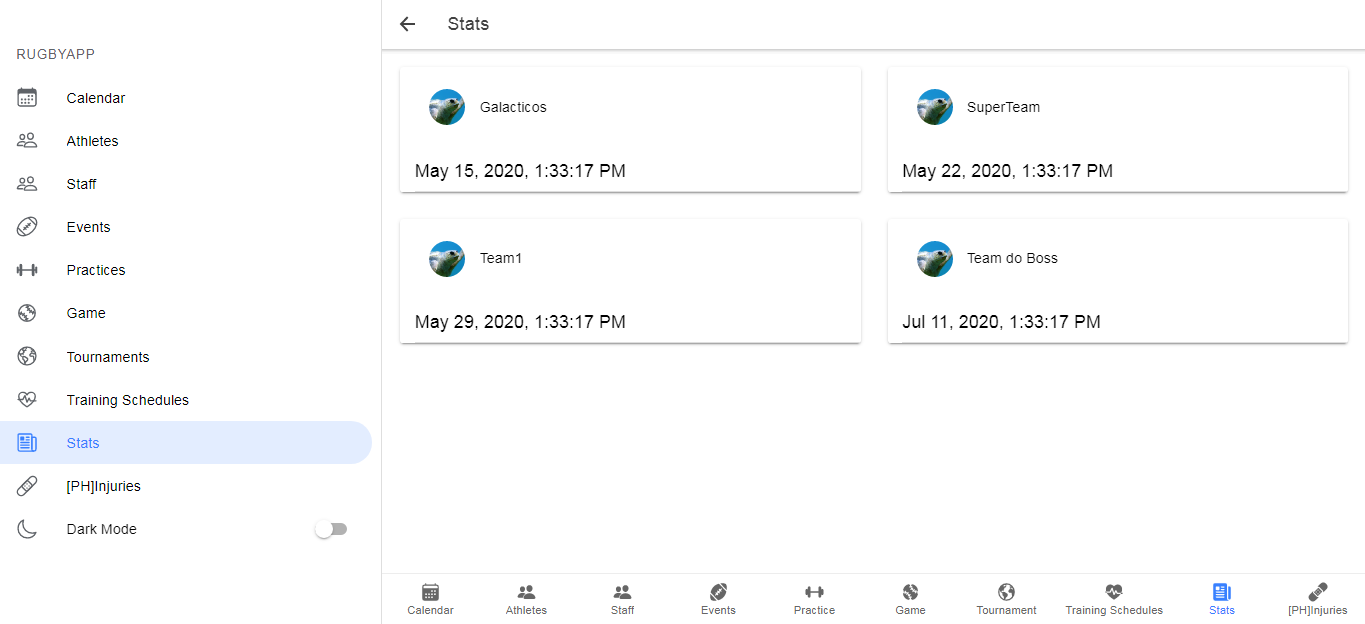
\includegraphics{./figures/frontend/StatsList.png}}
	\end{center}
	\caption{Página da lista de \textit{Games} do \textit{GameStats}.}\label{fig:gamestatslist}
\end{figure}

O menu de estatísticas de jogo apresenta uma lista de atletas associados ao jogo em contexto (\textbf{futuramente irá só apresentar os titulares}) e permite, para cada atleta, adicionar estatísticas. 

O utilizador pode clicar em qualquer um dos atletas na lista, e este atleta é apresentado na zona de \textit{selected} como o Atleta Ativo. Todas as estatísticas do menu são atualizadas com o valor das estatísticas deste atleta, e é possivel alterá-las. As estatísticas são alteradas através de botões que incrementam o valor da estatística. No caso de estatísticas \textit{Hit} e \textit{Miss}, existem dois botões para incrementar cada um. No meio de cada item de cada estatística está o nome da estatística e o valor (no caso de \textit{Hit} e \textit{Miss} mostra ambos), e no caso também de \textit{Hit} e \textit{Miss}, encontra-se do lado esquerdo a percentagem de sucesso. Cada estatística tem também um botão de \textit{Undo} (com as \textit{Hit} e \textit{Miss} a terem dois, um para \textit{Undo} de um \textit{Hit}, outro para \textit{Undo} de um \textit{Miss}). Estes botões existem para decrementar a estatística, em caso de erro humano.
\newpage

\begin{figure}[h]
	\begin{center}
		\resizebox{120mm}{!}{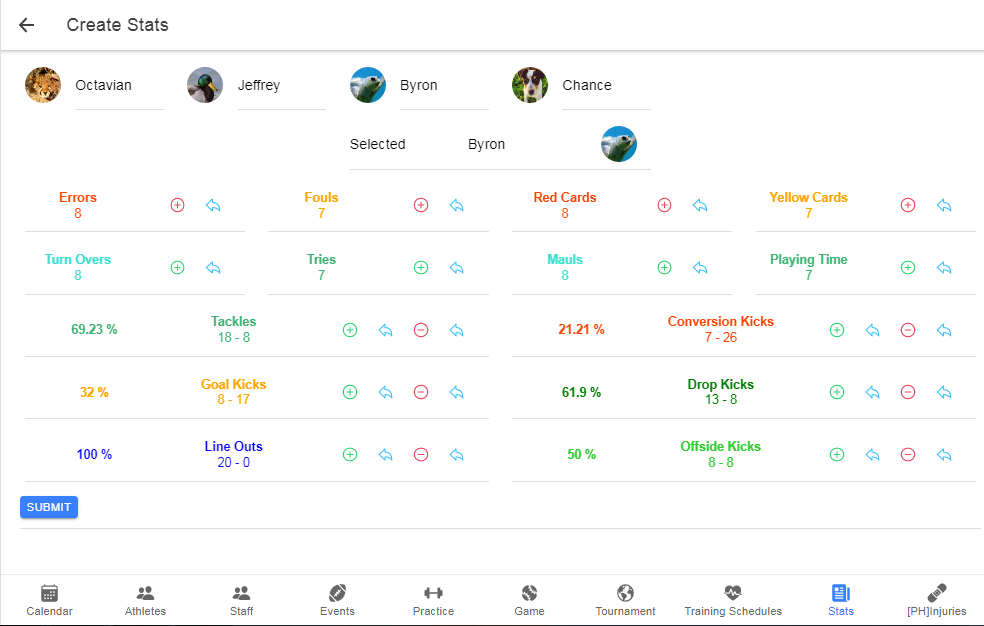
\includegraphics{./figures/frontend/GameStats2.png}}
	\end{center}
	\caption{Menu de estatísticas com o atleta "Byron" selecionado.}\label{fig:gamestatslist2}
\end{figure}

\begin{figure}[h]
	\begin{center}
		\resizebox{120mm}{!}{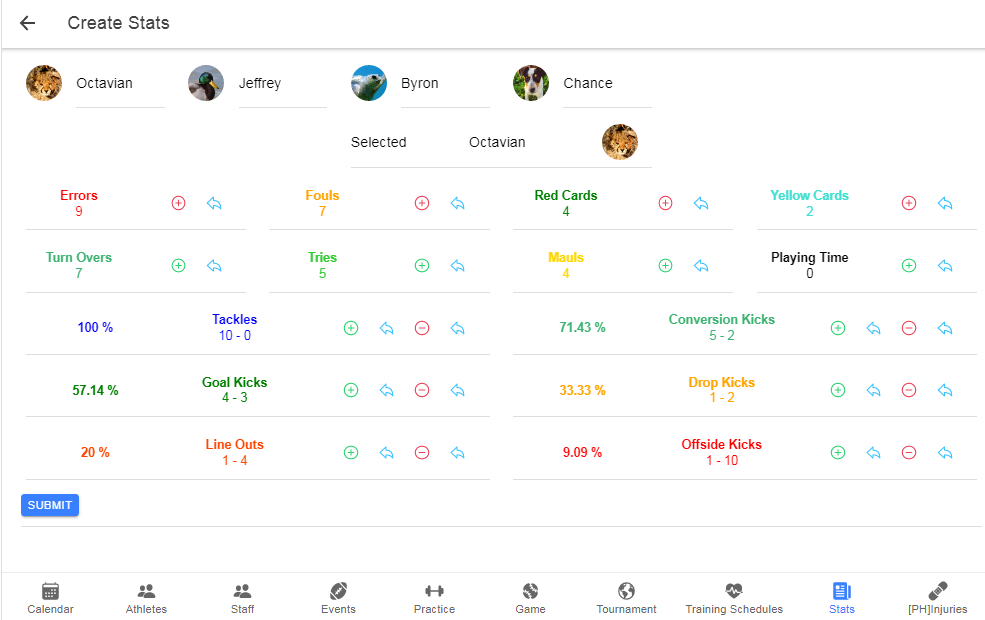
\includegraphics{./figures/frontend/GameStats.png}}
	\end{center}
	\caption{Menu de estatísticas com o atleta "Octavian" selecionado.}\label{fig:gamestatslist}
\end{figure}

Este menu apresenta um esquema de cores dinâmico. Como mencionado na sub-secção 4.1.3, é possível, através de um \textit{style binding}, alterar dinâmicamente o estilo de componentes \textit{HTML}. No serviço \textit{StatsService} foi definido um \textit{spectrum} (\textit{array} de \textit{strings} com valores de cores ordenados espectralmente), e cada valor de cada estatística altera a cor do texto do item para a cor indicada no \textit{spectrum}. Isto permite oferecer uma vertente visual às estatísticas de um jogador, dando uma percepção realista do seu desempenho sem considerar apenas os números. (\textbf{Este esquema está implementado estáticamente. O espectro de cores pode não corresponder à realidade de cada um, dado ser um tema emocional, e nem todos os jogos irão ter o mesmo grau de avaliação das estatísticas. Um jogo contra um oponente de nível inferior implica um maior peso negativo nos erros, e um jogo contra um oponente de nivel superior implica um menor peso negativo nos errors}).

\subsection{\textit{Forms}}\label{subsec428}
Os formulários são a principal maneira como o utilizador interage com a aplicação quando quer adicionar informação persistente (através dos \textit{endpoints} \textit{POST} ou \textit{PUT} da aplicação servidora). O formulário apresenta uma quantidade variável de campos com \textit{input} para o utilizador criar qualquer uma das entidades. 

No contexto da aplicação cliente, a nossa página dos formulários é a mesma para métodos de adicionar ou alterar uma entidade. No caso de o formulário ser acedido pelo \textit{update}, os campos do formulário são pré-preenchidos pelos valores atuais do objeto da entidade. Se for acedido pelo \textit{post}, os campos encontram-se vazios.
Isto concretiza-se utilizando o módulo \textit{ActivatedRoute} do \textit{Angular}, de onde é possível extrair variáveis do caminho que origina a criação do componente. Se o caminho contiver um \textit{id}, quer dizer que foi chamado no contexto de um objeto já existente, e por isso é um \textit{update} e vai, através da \textit{web API} da aplicação servidora, fazer \textit{fetch} desse objeto para pré-preencher os campos.

\begin{figure}[h]
	\begin{center}
		\resizebox{120mm}{!}{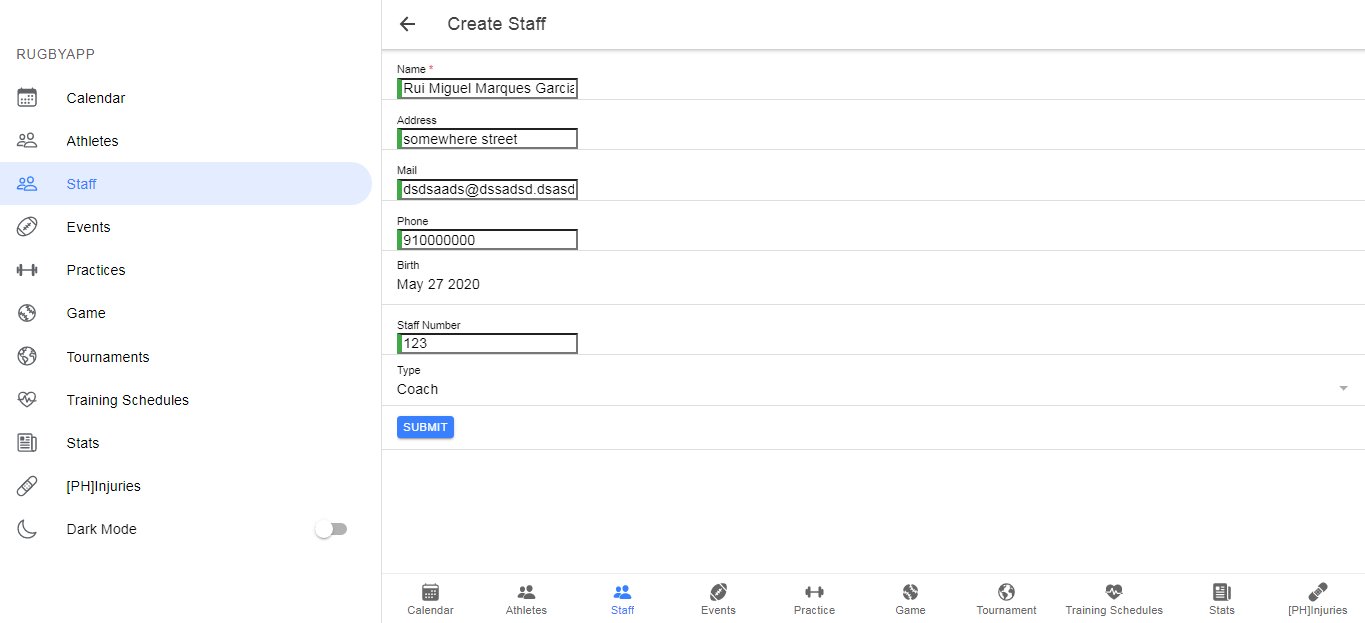
\includegraphics{./figures/frontend/FormUpdate.png}}
	\end{center}
	\caption{Formulário de um \textit{Staff} quando acedido através do botão \textit{Edit} da Lista de \textit{Staff}.}\label{fig:formupdate}
\end{figure}


São utilizados alguns componentes visuais da \textit{IONIC API} para garantir uma melhor experiência de utilizador no que toca a formulários\\

\begin{tabular}{ll}
	\textit{ion-select} & Explicado em detalhe na sub-secção 4.1.4\\
	\textit{ion-datetime} & Componente visual para se escolher datas. Em vez de ser escrita \\
	&manualmente, um \textit{click} num \textit{ion-datetime} abre um menu giratório onde \\
	&o utilizador pode através de \textit{scrolls} escolher os valores dos diversos \\
	&campos da data. 
	\\
\end{tabular}

Foi também utilizado, como referido na sub-secção 4.1.5, o componente \textit{mat-form-field} para criar as várias entradas dos formulários. Podemos observar, no exemplo seguinte, o troço de código \textit{HTML} do campo \textit{Height} do formulário de um atleta.

\begin{lstlisting}
<mat-form-field class="example-full-width" appearance="outline">
	<mat-label position="stacked"> Height </mat-label>
	<input matInput type="number"[(ngModel)]="athlete.height" name="height"
	pattern="[0-9]{1,3}" placeholder="Ex. 100">
	<button mat-button *ngIf="athlete.height" matSuffix mat-icon-button aria-label="Clear"
	(click)="athlete.height=''"> <mat-icon>x</mat-icon>
	</button>
	<mat-error>
	Please enter a valid value
	</mat-error>
</mat-form-field>
\end{lstlisting}

São observáveis, neste troço de código, todas as características importantes de um \textit{mat-form-field}, como o \textit{matInput}, o padrão necessário para o \textit{input} ser correto (3 dígitos entre 0 e 9), o botão no fim do campo para limpar o texto, o \textit{mat-error} que mostra em baixo, a vermelho, uma frase quando o \textit{input} está incorreto, e o \textit{placeholder}, que contem o texto que é mostrado quando o campo não tem nada escrito e está selecionado.

\begin{figure}[h]
	\begin{center}
		\resizebox{120mm}{!}{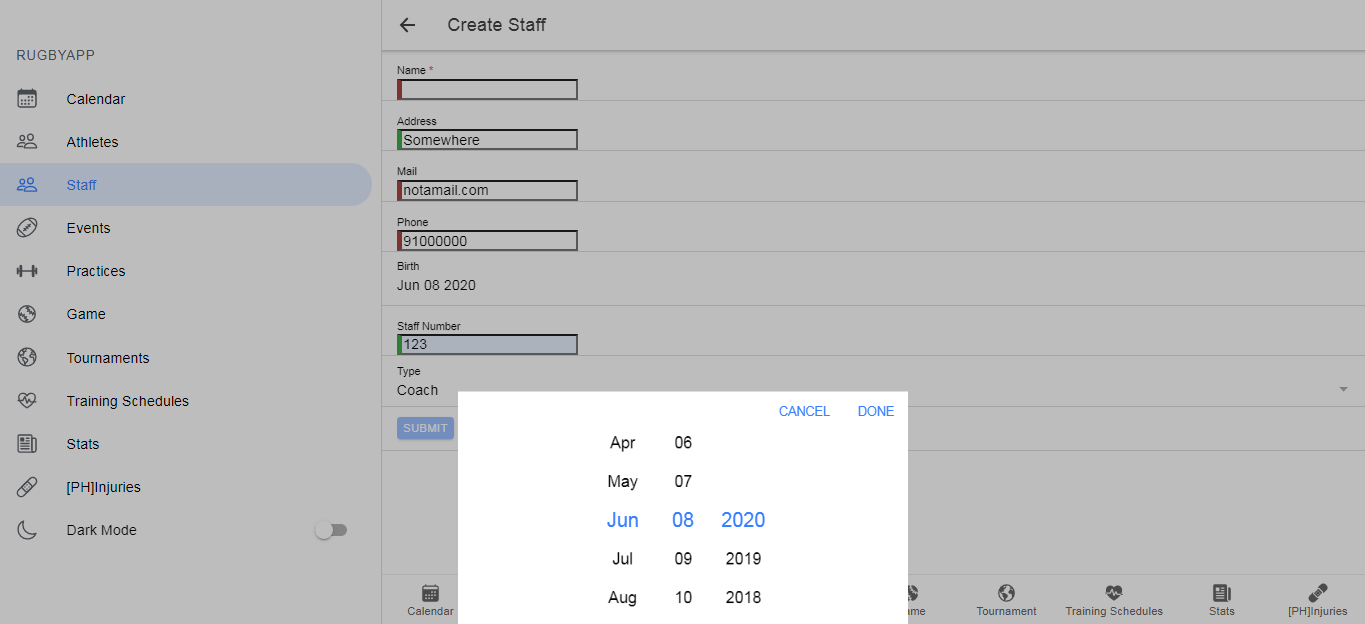
\includegraphics{./figures/frontend/FormPost.png}}
	\end{center}
	\caption{Formulário de um \textit{Staff} em preenchimento.}\label{fig:formpost}
\end{figure}

Podemos observar na figura 4.31 todos os aspetos importantes de um formulário. Os campos que são \textit{required} ficam a vermelho quando não estão preenchidos, os campos que têm padrões de escrita (um número de telefone requer pelo menos 9 digitos, um e-mail requer o padrão \textit{text@text.com}) ficam a vermelho quando o padrão não é cumprido corretamente. O botão \textit{submit} encontra-se \textit{disabled} pois os campos não estão todos corretos. Ao clicar na data de nascimento, abre-se o \textit{ion-datetime}, observável também na figura.


\subsection{\textit{[WIP]Injuries}}\label{subsec428}
A página de lesões ainda não se encontra implementada. Este tema representa uma especificação funcional que foi considerada anteriormente pelos elementos do grupo como secundária. No entanto, após algumas reuniões recentes com os clubes, foi decidido aumentar a prioridade desta especificação. Apesar de não haver ainda implementação para este tema, já foi possível aferir, através de uma reunião com o fisioterapeuta do Belas Rugby Clube, o modelo da entidade \textit{Injuries}.\\

\begin{tabular}{ll}
	AthleteInjury&\\
	&Lesão\\
	&Situação da lesão (inicial, em recuperação, recuperado)\\
	&Data de Inicio (mais virado para organização)\\
	&Data provisória de retorno do atleta\\
	&Recomendações do fisio (exercicios para fazer em casa, precausos)\\
	&\\
	Lesão&\\
	&Nome da Lesão\\
	&Zona Corportal (orgão, osso, músculo, etc)\\
	&Severidade (há lesões iguais com graus de severidade diferentes)\\
	&\\
\end{tabular}


Futuramente, este conceito irá ser inserido na aplicação servidora junto das outras entidades, e a aplicação cliente irá ter uma página com uma lista de lesões. Possivelmente o perfil de um atleta irá também conter alguma desta informação.
